\documentclass[12pt, a4paper, twocolumn]{article}

\usepackage[                            %
    a4paper,
    margin=0.5in,
    top=1in,
    bottom=1in
]{geometry}
\usepackage{fancyhdr}                   %
\usepackage{sectsty}                    %
\usepackage{graphicx}                   %

\usepackage{hyperref}
\usepackage{xcolor}

\newcommand{\toz}[1]{{\color{orange} [toz]: #1}}
\newcommand{\ajs}[1]{{\color{red} [ajs]: #1}}
\newcommand{\sd}[1]{{\color{blue} [sd]: #1}}
\newcommand{\nol}[1]{{\color{purple} [nol]: #1}}

\newcommand{\descr}{\emph}

\title{Reward Report - MuZero}
\author{DeepMind}

\graphicspath{
    {./figures/}
}

\setlength{\columnsep}{0.5in}

\sectionfont{\fontsize{14}{16}\selectfont}
\subsectionfont{\fontsize{12}{14}\selectfont}

\pagestyle{fancy}
\fancyhf{}
\lhead{Reward Report: MuZero Gameplaying AI}
\rhead{Page \thepage}



\newcommand{\descr}{\small \emph}
\newcommand{\eg}{\textit{e.g.}}             % For example
\newcommand{\etc}{\textit{etc}.}           % So on...
\newcommand{\ie}{\textit{i.e.}}             % literally


\newcommand{\SystemDetails}[4]{
\section{System Details}
\subsection{System Owner}
\descr{This may be the designer deploying the system, a larger agency or body, or some combination of the two. The entity completing the report should also be indicated.}

#1
% % % % % 
\subsection{Dates}
\descr{The
known or intended timespan over which this reward function \& optimization is active. }

#2
% % % % % 
\subsection{Feedback \& Communication}
\descr{Contact information for the designer, team, or larger agency responsible for system deployment.}

#3
% % % % % 
\subsection{Other Resources}
\descr{Where can users or stakeholders find more information about this system? Is this system based on one or more research
papers?}

#4
}

% % % % % % % % % % 
\newcommand{\OptIntent}[4]{
\section{Optimization Intent}
\subsection{Goal of Reinforcement}
\descr{A statement of system scope and purpose, including the planning horizon and justification of
a data-driven approach to policy design (\eg{} the use of reinforcement learning or repeated retraining). This justification
should contrast with alternative approaches, like static models and hand-designed policies. What is there to gain with
the chosen approach?}

#1
% % % % % 
\subsection{Defined Performance Metrics}
\descr{A list of “performance metrics” included explicitly in the reward
signal, the criteria for why these metrics were chosen, and from where these criteria were drawn (\eg{} government
agencies, domain precedent, GitHub repositories, toy environments). Performance metrics that are used by the designer
to tune the system, but not explicitly included in the reward signal should also be reported here.}

#2
% % % % % 
\subsection{Oversight Metrics}
\descr{Are there any additional metrics not included in the reward signal but relevant for vendor or system oversight (e.g.
performance differences across demographic groups)? Why aren’t they part of the reward signal, and why must they
be monitored? }

#3
% % % % % 
\subsection{Known Failure Modes}
\descr{A description of any prior known instances of “reward hacking” or model
misalignment in the domain at stake, and description of how the current system avoids this.}


#4
}

% % % % % % % % % % 
\newcommand{\Interfaces}[4]{
\section{Institutional Interface}
\subsection{Deployment Agency}
\descr{ What other agency or controlling entity roles, if any, are intended to be subsumed by the
system? How may these roles change following system deployment?}

#1
% % % % % 
\subsection{Stakeholders}
\descr{What other interests are implicated in the design specification or system deployment, beyond the designer? What role will these interests play in
subsequent report documentation? What other entities, if any, does the deployed system interface with whose interests
are not intended to be in scope? }

#2
% % % % % 
\subsection{Explainability \& Transparency}
\descr{Does the system offer explanations of its decisions
or actions? What is the purpose of these explanations? To what extent is the policy transparent, \ie{} can decisions or
actions be understood in terms of meaningful intermediate quantities? }

#3
% % % % % 
\subsection{Recourse}
\descr{Can stakeholders or users contest
the decisions or actions of the system? What processes, technical or otherwise, are in place to handle this?}

#4
}

% % % % % % % % % % 
\newcommand{\Implementation}[7]{
\section{Implementation}
\subsection{Reward Details}
\descr{How was the reward function engineered? Is it
based on a well-defined metric? Is it tuned to represent a specific behavior? Are multiple terms scaled to make one
central loss, and how was the scaling decided?}

#1
% % % % % 
\subsection{Environment Details}
\descr{Description of states, observations, and actions
with reference to planning horizon and hypothesized dynamics/impact. What dynamics are brought into the scope of
the optimization via feedback? Which dynamics are left external to the system, as drift? Have there been any observed
gaps between conceptualization and resultant dynamics?}



#2
% % % % % 
\subsection{Measurement Details}
\descr{How are the components of the
reward and observations measured? Are measurement techniques consistent across time and data sources? Under what
conditions are measurements valid and correct? What biases might arise during the measurement process? }

#3
% % % % % 
\subsection{Algorithmic Details}
\descr{The key points on the specific algorithm(s) used for learning and planning. This includes the form of the
policy (\eg{} neural network, optimization problem), the class of learning algorithm (\eg{} model-based RL, off-policy RL,
repeated retraining), the form of any intermediate model (\eg{} of the value function, dynamics function, reward function),
technical infrastructure, and any other considerations necessary for implementing the system. Is the algorithm publicly
documented and is code publicly available? Have different algorithms been used or tried to accomplish the same goal?}

#4
% % % % % 
\subsection{Data Flow}
\descr{How is data collected, stored, and used for (re)training? How frequently are various components of the
system retrained, and why was this frequency chosen? Could the data exhibit sampling bias, and is this accounted for in
the learning algorithm? Is data reweighted, filtered, or discarded? Have data sources changed over time?}

#5
% % % % % 
\subsection{Limitations}
\descr{Discussion and justification of modeling choices arising from computational, statistical, and measurement limitations.
How might (or how have) improvements in computational power and data collection change(d) these considerations
and impact(ed) system behavior?}

#6
% % % % % 
\subsection{Engineering Tricks}
\descr{RL systems are known to be sensitive to implementation tricks
that are key to performance. Are there any design elements that have a surprisingly strong impact on performance? For example,
state-action normalization, hard-coded curricula, model-initialization, loss bounds, or more?}

#7
}

% % % % % % % % % % 
\newcommand{\Evaluation}[4]{
\section{Evaluation}
\subsection{Evaluation Environment}
\descr{ How is the system evaluated (and if applicable, trained) prior to deployment (\eg{} using
simulation, static datasets, \etc{})? Exhaustive details of the offline evaluation environment should be provided. For simulation, details should
include description or external reference to the underlying model, ranges of parameters, etc. 
For evaluation on static datasets, considering referring to associated documentation (\eg{} \emph{Datasheets}~\cite{gebru2021datasheets}).
}

#1
% % % % % 
\subsection{Offline Evaluations}
\descr{Present and discuss the results of offline
evaluation. 
For static evaluation, consider referring to associated documentation (\eg{} \emph{Model Cards}~\cite{mitchell2019model}).
If applicable, compare the behaviors arising from counterfactual specifications
(e.g. of states, observations, actions). }

#2
% % % % % 
\subsection{Evaluation Validity}
\descr{ To what extent is it reasonable to draw conclusions about
the behavior of the deployed system based on presented offline evaluations? What is the current state of understanding
of the online performance of the system? If the system has been deployed, were any unexpected behaviors observed?}

#3
% % % % % 
\subsection{Performance standards}
\descr{What standards of performance and safety is the system required to meet? Where do these
standards come from? How is the system verified to meet these standards?}

#4

% \descr{Evaluation of simulated behaviors as well as exhaustive details on simulation parameters. This can include the timestep used in simulation, underlying world model, computational software used, external references,
% and any more relevant information. Was the model developed in a closed simulation? Are there plans for transferring
% from sim to real? Is the deployed environment exactly the same as the training environment?}


% \descr{Is the implementation centered around finding a solution or recreating a known solution to
% a problem? Has the environment been modified to make the task easier? Is there an existence of a predetermined
% "optimal" behavior?}

% \descr{The state of understanding the quantified performance of the initial agent used by the system.
% Were the observed behaviors expected?}
}

% % % % % % % % % % 
\newcommand{\Maintenance}[3]{
\section{System Maintenance}
\subsection{Reporting Cadence}
\descr{The intended
timeframe for revisiting the reward report. How was this decision reached and motivated? }

#1
% % % % % 
\subsection{Update Triggers}
\descr{Specific
events (projected or historic) significant enough to warrant revisiting this report, beyond the cadence outlined above.
Example triggers include a defined stakeholder group empowered to demand a system audit, or a specific metric (either
of performance or oversight) that falls outside a defined threshold of critical safety.}

#2
% % % % % 
\subsection{Changelog}
\descr{Descriptions of updates
and lessons learned from observing and maintaining the deployed system. This includes when the updates were made
and what motivated them in light of previous reports. The changelog comprises the central difference between reward
reports and other forms of machine learning documentation, as it directly reflects their intrinsically dynamic nature.}


#3


}



\begin{document}



\SystemDetails
{This system was developed by the DeepMind
core Reinforcement Learning Team members.
More information about AlphaGo's development can be found at the project website (https://deepmind.com/research/case-studies/alphago-the-story-so-far) as well as DeepMind's GitHub repository}
{Development of AlphaGo began about two years prior to the matches against Lee Sedol in spring 2016, shortly after DeepMind's acquisition by Google \cite{pcworld}.
Development of AlphaZero, based entirely on self-play, followed AlphaGo and was completed prior to October 2017.
Development of MuZero, also based on self-play, followed AlphaZero and was first described in a preliminary paper in 2019 \cite{schrittwieser2020mastering}. }
{Any correspondence should be directed to
\url{press@deepmind.com.}}
{There is little additional disclosed information.}

\OptIntent
{Go, and general game-playing at a human level, was long defined as one of the ``grand challenges'' of AI. 
For AlphaGo, the use of reinforcement to learn both the policy and value networks beyond the abilities of a human expert. %

For AlphaZero, the sole use of reinforcement learning without any human data was important validation of its potential as a more general learning procedure \cite{silver2017mastering}.
The algorithm additionally incorporated lookahead search (Monte Carlo Tree Search) inside the training loop.

For MuZero, the use of model-based reinforcement learning without any prior knowledge of the game dynamics was further indication of RL's potential to develop planning capabilities in more challenging or complex domains \cite{schrittwieser2020mastering}.
The learned model performed well in both classic game environments (Go, chess, shogi) as well as canonical video game environments (57 distinct Atari games).}
{As with most game-playing systems, the performance metric is defined as a win rate among games.
In other games, score is used, but in one-versus-one games win rate is the only direct metric.
To better capture the uncertainty of playing varying opponents, this win rate is translated into a running Elo rating system.}
{Some other performance metrics are not included in the specification, but are monitored for the purpose of evaluating system effects on the domain:

\begin{itemize}
    \item Absolute opponents' world rankings - following their public games, versions of AlphaGo and AlphaZero were considered to possibly improve the skill levels of expert human opponents, as measured by those players' absolute world ranking.
    If humans played better after playing AlphaGo, this was to be seen as a positive effect of the system's influence on the game of Go.
    Fan Hui, following his games against AlphaGo, claimed it made him a better played and accredits his world ranking jump from 600 to 300 in three months to training against it \cite{fan}.
    \item Qualitative changes in playstyle - following their public games, versions of AlphaGo were considered to possibly  influence the playstyle of expert human opponents, as interpreted by the wider community of expert players.
    If expert humans played differently, more creatively or unpredictably, or expressed surprise after AlphaGo's public performances, this was to be seen as a positive effective of the system's influence on the game in question.
    Garry Kasparov, following his observation of AlphaZero play, was impressed that it appeared to be ``a very sharp and attacking player'' given that almost all computer programs have a conservative playstyle \cite{kasparov}.
    While not integral in any way for system performance, AlphaGo's performance and playstyle have had a noticeable impact on the strategies of expert human players.
\end{itemize}}


{\textit{Monte Carlo search limitations.} In the fourth match (of five) against Lee Sedol in spring 2016, the system failed to recognize move 78 by Sedol. 
The Monte Carlo search tree, which was designed to prune sequences of moves considered to be irrelevant for maximizing odds of victory, failed to recognize this move.
This is because that move was so far outside the distribution of prior game situations that the AlphaGo system failed to accurately calculate its significance for determining the odds of victory \cite{montecarlo}. 
The result was a sequences of moves 79-87 by AlphaGo that were considered poor by expert human players, a function of Monte Carlo's myopic look-ahead search following move 78.
AlphaGo subsequently conceded the game at move 178, at which point it evaluated its own odds of victory as lower than 20 percent \cite{game4}.}

\Interfaces
{The AlphaGo system was developed by DeepMind.
This version played against Fan Hui in 5 matches held at DeepMind headquarters in October 2015.
These matches were secret and not revealed until the publication of results in January 2016 \cite{silver2016mastering}.
A later version of the same system, AlphaGo Lee, played Lee Sedol in March 2016 in 5 matches in Seoul, South Korea.
This match was overseen by the Korea Baduk Association.
A yet more sophisticated version of the same system, AlphaGo Master, played against Ke Jie at the Future of Go Summit in Wuzhen, China in May 2017.
An earlier version of AlphaGo Master, dubbed Master, had already won 60 straight online games against top pro players, including against Ke Jie \cite{master}.
This version was awarded a professional 9-dan title by the Chinese Weiqi Assocation.}
{Compared to other prominent automated game-playing systems like Stockfish (open-source chess engine) or CrazyStone (offline Go engine based on deep learning), versions of AlphaGo perform much much better with additional computational power.
The versions of AlphaGo that played against Fan Hu, Lee Sedol, and Ke Jie all made use of distributed CPUs and GPUs.
AlphaGo Zero, based entirely on reinforcement learning and self-play, became stronger than AlphaGo Lee after 3 days and stronger than AlphaGo Master after 21 days.
Its self-play training time was stopped after 40 days, at which point it was stronger than any known Go player (human or program) as measured by Elo rating in October 2017 \cite{master}.

AlphaZero, in its initial chess games against Stockfish, was criticized by expert human chess players has having unfair computational advantages over the opponent \cite{stockfish}.

MuZero's learning has been made more efficient in follow-up work, dubbed EfficientZero \cite{ye2021mastering}.}
{The MuZero system offers few tools for transparency in its current form. 
While the learning process develops a structured model for the game dynamics, it is not done in a way that is accessible by engineers or external parties.}
{N/A}

\begin{figure}[t]
    \includegraphics[width=0.47\textwidth]{figures/Alphago.png}
    \caption{%
        The AlphaGo game playing system architecture.
    }
\end{figure}

\begin{figure}[t]
    \includegraphics[width=0.47\textwidth]{figures/alphazero.png}
    \caption{%
        The AlphaZero game playing system architecture.
    }
\end{figure}

\begin{figure}[t]
    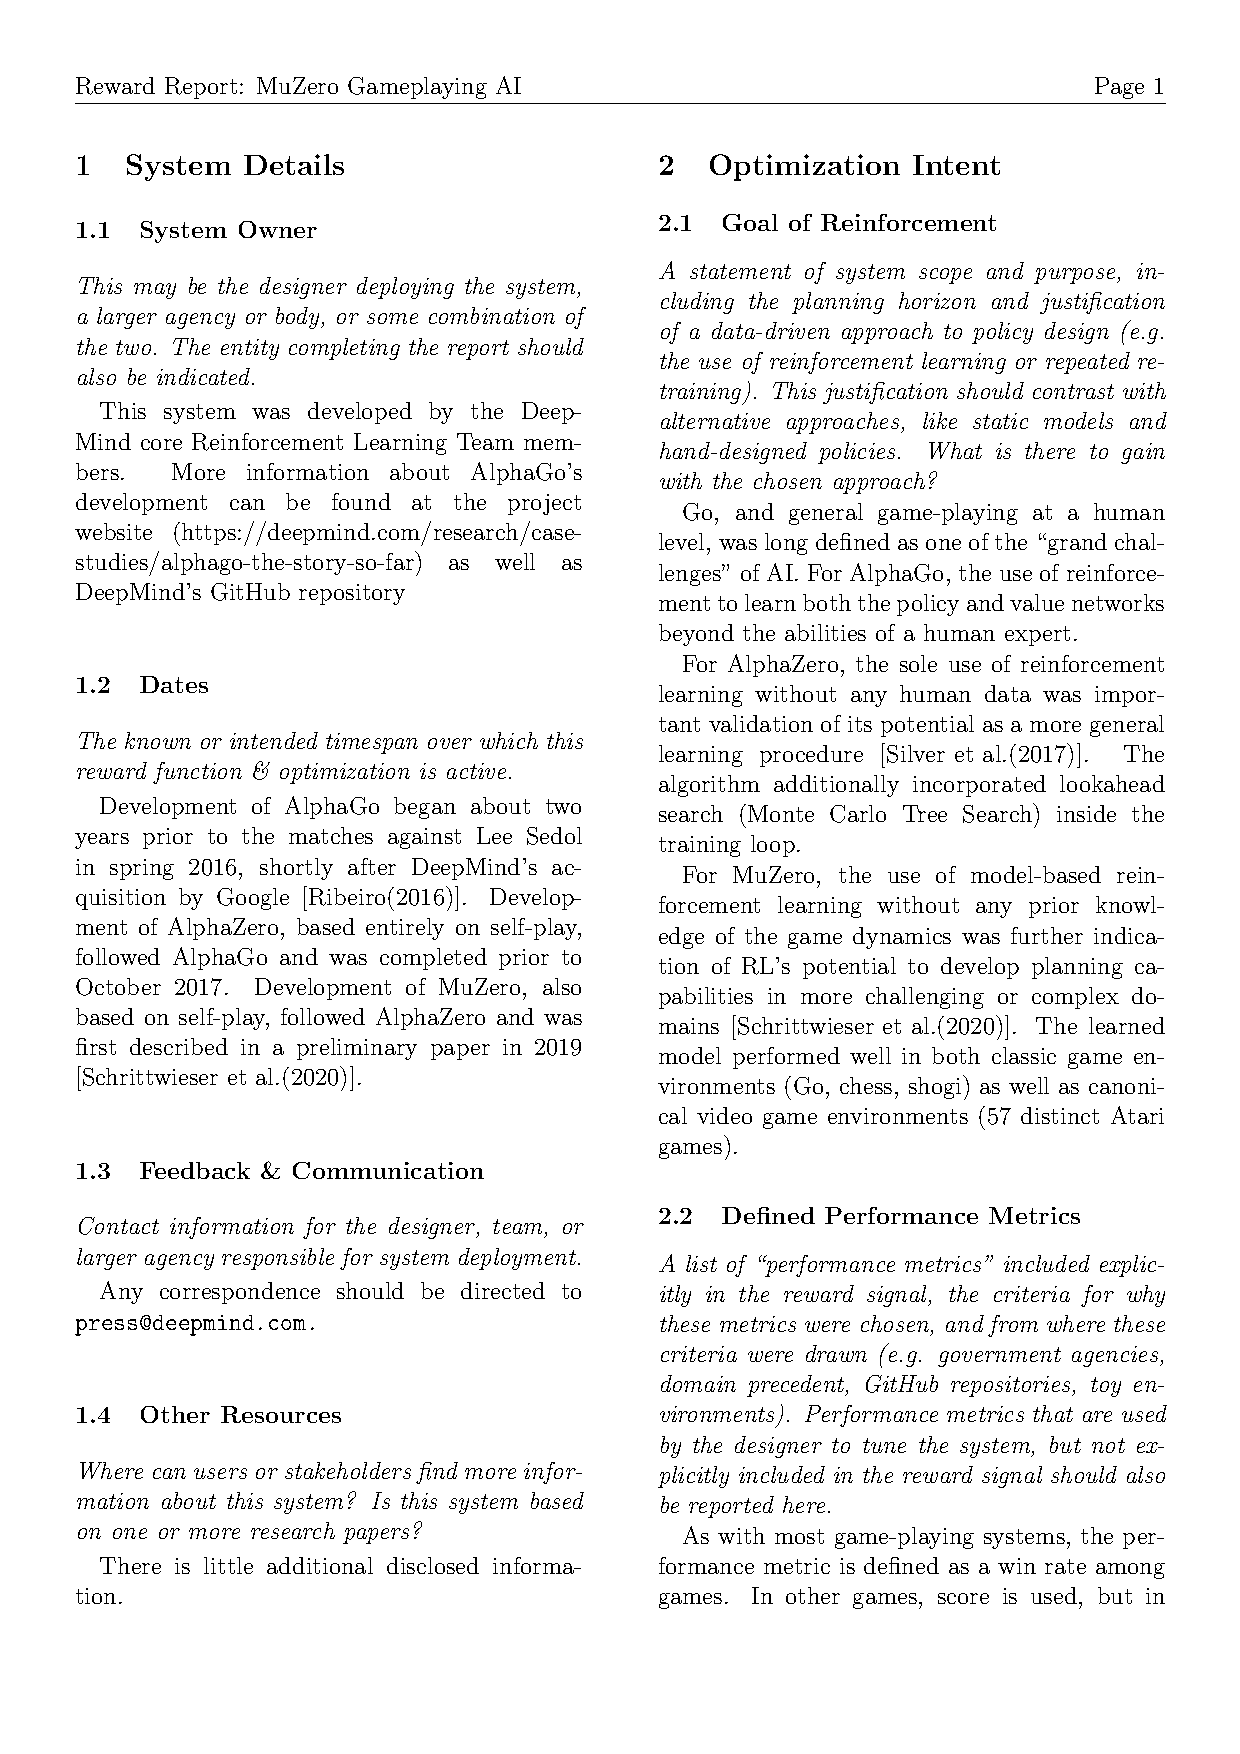
\includegraphics[width=0.47\textwidth]{figures/muzero.png}
    \caption{%
        The MuZero general game playing system.
    }
\end{figure}

\begin{figure}[t]
    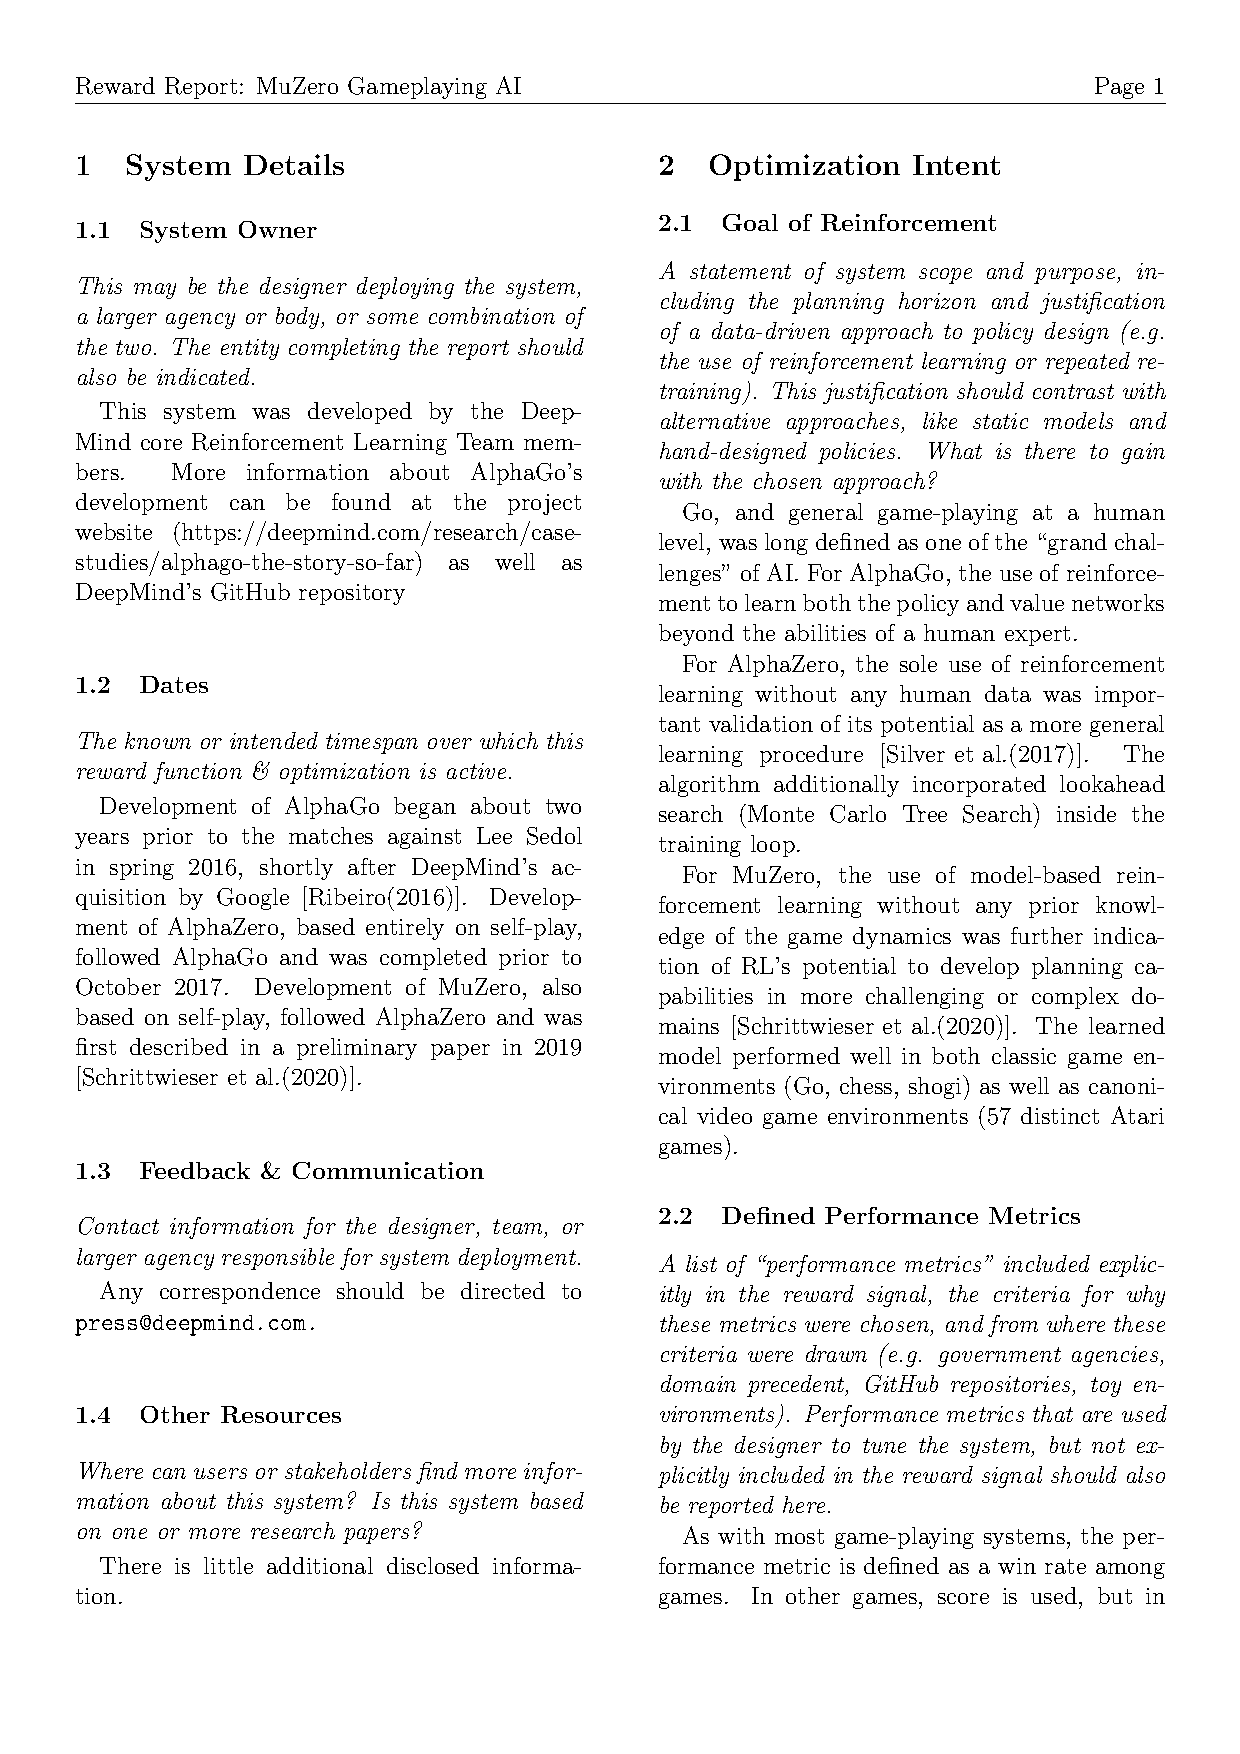
\includegraphics[width=0.47\textwidth]{figures/muzero.png}
    \caption{%
        The MuZero general game playing system.
    }
\end{figure}
\Implementation
{The reward function is entirely prescribed as win rate, and the resulting Elo rating.
An important sub-component that will be referenced later is the value function estimating game state. 
This is an internal representation of reward central to training and evaluation. }
{The original environment is the full game of Go which is constrained by finite rules, but other games with visual states were added.}
{The measurements differ across games from the full gameboard to a visual rendering of the world. 
Extracting information from pixels is substantially less efficient than directly from the game state.}
{The key algorithm feature is the use of Monte Carlo Tree Search (MCTS). 
MCTS is used to search over board states (by planning over actions) and parses the value representation.
The value function is represented by a deep neural network mapping from game state to value.

The second crucial element to training is self play. 
Here gameplaying agents evaluate their performance versus past training snapshots.
This synergistic mechanism is crucial to reaching superhuman performance.
In MuZero, and learned model is used to used to improve performance in games without complete information (such as visual states) by constraining the policy optimization.
At each turn, the model is used to predict the correct policy, the value function, and the reward received by the move (in games that have an intermediate score).
The model is updated in an end-to-end fashion, so it is included in the same training loop in the agent architecture.

Fully algorithmic details and open source code are not released.}
{Data flow is not well documented, but it relies on Google's distributed training and deployment infrastructure.}
{}
{Not documented.}

\Evaluation
{For games, the simulator is reality so evaluation is matched to training.
}
{Multiple internal evaluations of the agent were performed prior to high-profile, public matches with the worlds best players. 
}
{}
{N/A.}

\Maintenance
{While this system is evaluated in closed-world games, updates are not anticipated.}
{This report will be revisited upon release of each new game-playing AI from DeepMind.}
{N/A (v1)}









\bibliographystyle{ACM-Reference-Format}
\bibliography{main}

\end{document}